\chapter{Estado del arte}
\label{estadoArte}

En el presente capítulo se entrará en profundidad en los conceptos más relevantes relacionados con el \gls{tfm}. Además, se describirán las diversas herramientas de software que se emplearán. El propósito principal de presentar el estado del arte es establecer un marco teórico consistente que permita conseguir una mayor compresión del contexto previamente a la exposición del desarrollo del proyecto.


% %%%%%%%%%%%%%%%%%%%%%%%%%%%%%%%%%%%%%%%%%%%%%%%%%%%%%%%%%%%%%%%%%%%%%%%%%%%%%%%%%%%%%%%%%%%%%%%%%%%%%
%%%%%%%%%%%%%%%%%%%%%%%%%%%%%%%%%%%%%%%%%%%%%%%%%%%%%%%%%%%%%%%%%%
\section{Smart Grids}
\label{sec:smartgrids}


En las últimas décadas, se ha observado una transformación integral del modelo asociado a la red eléctrica convencional. El aumento de la energía demandada por los usuarios finales y los requisitos cada vez mayores de la industria ha tenido como consecuencia que algunos países hayan intentado diseñar redes eléctricas agrupadas en un conjunto de grandes redes nacionales. De este modo, todas las fuentes energéticas disponibles pueden estar conectadas para ser gestionadas conjuntamente en función de la demanda recibida, además de conseguir una coordinación a alto nivel. \cite{smartgrid_overview}

\vspace{3mm}

Sin embargo, una red eléctrica no se puede definir como una entidad única e independiente, pues se trata de una agregación de redes, compañías energéticas y operadores que trabajan en distintos niveles de comunicación. Es por ello, que la idea de desarrollar una gran red nacional encuentra cierto equilibrio energético, pero no llega a los altos porcentajes de eficiencia que pueden proveer las redes inteligentes energéticas o de otra forma, las \textit{smart grids} (\gls{sg}). 

\vspace{3mm}

La iniciativa sobre redes inteligentes del \gls{ieee}, califica a las \textit{smart grids} \cite{ieee} como "imperativas y revolucionarias que implican nuevas capacidades de comunicación y control, fuentes de energía, modelos de generación y adherencia a estructuras regulatorias transjurisdiccionales". Por otro lado, en el año 2009, el Departamento de Energía de Estados Unidos \cite{us} determinó en su reporte anual sobre \textit{smart grids} los siguientes objetivos principales que se perseguían con el desarrollo de este tipo de redes: 

\pagebreak

\begin{itemize}
  \item Permitir una participación activa de los clientes en el sistema.
  \item Integrar todas las opciones de generación y almacenamiento de energía.
  \item Ofertar nuevos productos y servicios.
  \item Proporcionar energía de calidad y satisfacer un gran rango de necesidades.
  \item Optimizar el uso de los recursos y aumentar la eficiencia.
  \item Dar una respuesta rápida ante emergencias y problemas producidos en la red.
\end{itemize}

\vspace{1mm}

Teniendo estos objetivos en cuenta, se puede definir una \textit{smart grid} como una red inteligente con la capacidad de distribuir los suministros de energía de forma optimizada a los usuarios, basándose en la información que recoge de los mismos. Es por ello que supone una actualización digital de las redes de distribución y transmisión a larga distancia para incorporar sistemas de monitorización y control a tiempo real. \cite{iotfutura} 

\vspace{3mm}

Su base se asienta en el diseño de sistemas inteligentes coordinados capaces de obtener tanto la información respectiva a la demanda o requisitos energéticos de cada zona como la de la disponibilidad de recursos a partir de las diferentes fuentes de producción existentes. Todo ello conduce al desarrollo de un plan estratégico de distribución energética para poder conectar a todas las entidades participantes en la red entre sí. \cite{repsol}

\vspace{1mm}

%%%%%%%%%%%%%%%%%%%%%%%%%%%%%%%%%%%%%%%%%%%%%%%%%%%%%%%%%%%%%%%%%%
\subsection{Flujo energético y comunicación bidireccional}

Cabe destacar que una de las principales características diferenciadoras de las \gls{sg}s respecto a las redes energéticas convencionales es que se fundamentan en una comunicación bidireccional. Este factor determinante se puede apreciar en la Figura \ref{fig:bidireccional} y se traduce en una producción y una distribución dinámica y personalizada hacia cada usuario de la red. 

\begin{figure}[h!]
  \centering
  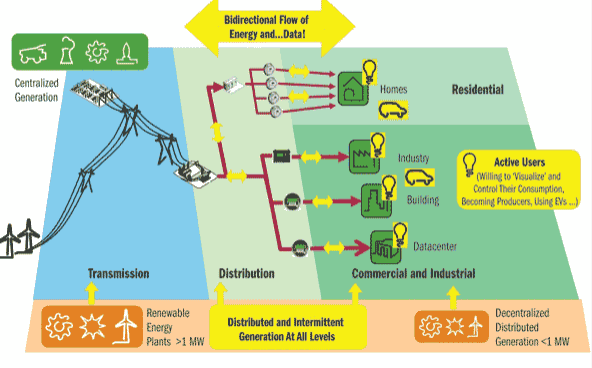
\includegraphics[width=0.9\textwidth]{img/teoria/sg.png}
  \caption{Flujo bidireccional de datos y energía en una \textit{smart grid} \cite{sins}}
  \label{fig:bidireccional}
\end{figure}

\vspace{3mm}

\begin{figure}[h!]
  \centering
  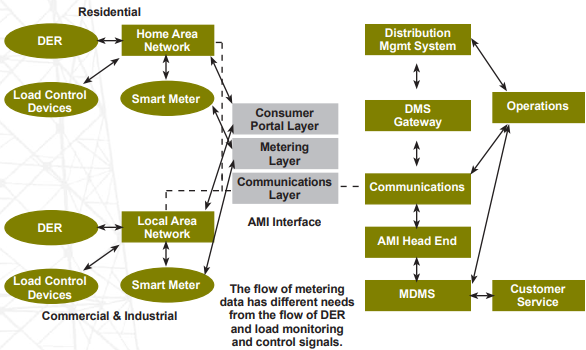
\includegraphics[width=0.9\textwidth]{img/teoria/bidir.png}
  \caption{Infraestructura de una interfaz \gls{ami} para el flujo bidireccional de energía y datos \cite{us}}
  \label{fig:bidireccional2}
\end{figure}

Es decir, en una red tradicional al ser unidireccional, se provee energía desde el distribuidor hacia el consumidor sin llevar a cabo ningún análisis estadístico sobre el consumo que se está produciendo en las líneas finales en un determinado instante temporal. En cambio, en el contexto de las \gls{sg}s, se pone el foco en las acciones de los usuarios y en la consecuente asignación de patrones de consumo eléctrico que permita predecir el comportamiento futuro de los mismos. \cite{convencional}

\vspace{3mm}

Sin embargo, como se expondrá más adelante en la Sección \ref{sec:consumo}, este proceso de clasificación de usuarios requerirá del análisis de grandes volúmenes de datos adquiridos a tiempo real, por lo que se aumentará la complejidad del sistema a costa de alcanzar la eficiencia.

\vspace{3mm}

Por lo tanto, teniendo en cuenta la característica de red bidireccional, se puede expresar que los propios usuarios son el gran pilar sobre el que se cimienta el sistema. En comparación a la red eléctrica tradicional, toman un papel mucho más activo monitorizando continuamente su comportamiento eléctrico y recopilando información para trasladarla al resto de la red. Esto tiene como ventaja una gran reducción de los costes derivados de la distribución y transmisión en el sistema, ya que se evita proporcionar más cantidad de energía de la requerida por las líneas finales. \cite{iotfutura}

\vspace{3mm}

Es por ello que se emplea una Infraestructura Avanzada de Medición (del inglés \gls{ami}) con una interfaz constituida por varias capas o niveles como se puede apreciar en la Figura \ref{fig:bidireccional2}. De esta forma, se dividen los flujos de comunicación entre las diferentes entidades que componen la red para permitir una mejor gestión de los mismos. \cite{us}

\vspace{1mm}

%%%%%%%%%%%%%%%%%%%%%%%%%%%%%%%%%%%%%%%%%%%%%%%%%%%%%%%%%%%%%%%%%%
\subsection{Prosumidores y microgrids}
\label{sec:prosu}

Dentro del presente contexto, en referencia a los usuarios es preciso introducir el término de prosumidor \cite{prosumer}. Se puede determinar como prosumidora a toda entidad o usuario final que tiene la capacidad de producir de forma alternativa recursos energéticos, además de poder consumirlos. En la Figura \ref{fig:prosumer} se puede visualizar cómo se estructura la \gls{sg} en un conjunto de distintas comunidades o agregaciones de prosumidores con el fin de crear microrredes de distribución y almacenamiento energético (del inglés \textit{microgrids}).

\begin{figure}[h!]
  \centering
  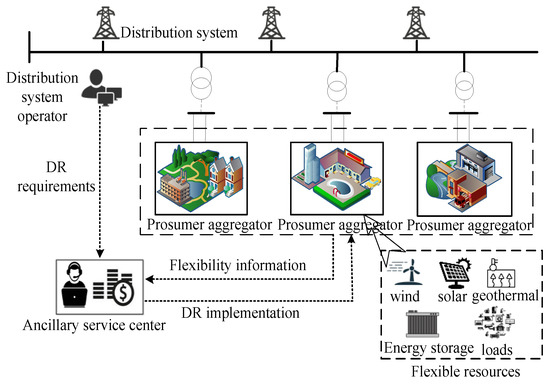
\includegraphics[width=1\textwidth]{img/teoria/prosumer.jpg}
  \caption{Estructura de la respuesta a la demanda en el contexto de una \textit{smart grid} con prosumidores \cite{prosumer}}
  \label{fig:prosumer}
\end{figure}

En este caso es imprescindible que los equipos y dispositivos dedicados a la generación de electricidad se encuentren dentro de la microrred o en una ubicación cercana a la misma. Así, se podrá abastecer a los usuarios del conjunto de forma eficiente, reduciendo los costes relacionados con la transmisión energética. 

\vspace{3mm}

Este tipo de esquema puede ser aplicado en diferentes entornos, como pueden ser los residenciales, industriales o agrícolas, para conseguir descentralizar la gestión de los recursos. Sin embargo, debe existir cierta gestión externa y coordinada de todas estas microrredes o comunidades de usuarios. Esta es llevada a cabo por una entidad denominada como operador del sistema distribuido (del ingles \gls{dso}) \cite{transactive} \cite{dso}. Algunas de sus funciones principales se basan en asegurar el abastecimiento de recursos en el interior de las microrredes en función de la demanda existente y en supervisar el estado operativo la infraestructura de red para garantizar su estabilidad y seguridad. 

\vspace{3mm}

Por otro lado, se encuentra también la figura del centro de servicios auxiliares \cite{transactive}, que se encarga de recibir la información sobre los recursos energéticos de los prosumidores y cuantificar en función de la oferta y demanda el beneficio económico que obtendrán los prosumidores. Estos normalmente son gestionados por los operadores del mercado eléctrico, pero puede variar según la región o el país.

\vspace{3mm}

\subsubsection{Mercado energético}

Las agregaciones de prosumidores posibilitan el autoconsumo y la compartición de los recursos generados por sí mismos con los demás participantes de la microrred, incluso con el resto de la \gls{sg}. La mayoría de los prosumidores, sobre todo en entornos residenciales son de pequeño tamaño y tienen mayores complicaciones para participar en los mercados eléctricos por sí mismos. 

\vspace{3mm}

Por ello, los agregadores \cite{bidding} \cite{transactive} se encargan de facilitar esta tarea para que una cantidad de prosumidores locales puedan actuar en conjunto como fijadores de precios de compra/venta en el mercado eléctrico global. Es decir, cada agregador se encarga de representar a los prosumidores que lo componen y actúa como intermediarios entre los mismos y el conjunto de mercados energéticos. 

\vspace{3mm}

A cambio, cada prosumidor debe pagar un plan mensual a la compañía para cubrir los costes eléctricos y así, dejar la responsabilidad de las transacciones a los agregadores para que operen de forma flexible. En esta operativa también incide el \gls{dso}, el cual se encarga de que las transacciones de compra/venta sigan el cumplimiento de los estándares y regulaciones establecidos en el mercado energético. 
\vspace{3mm}

\begin{figure}[h!]
  \centering
  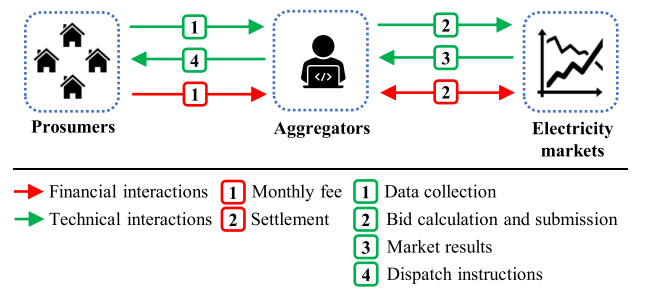
\includegraphics[width=0.9\textwidth]{img/teoria/market.png}
  \caption{Modelo basado en las interacciones de los agregadores con los prosumidores y el mercado eléctrico \cite{business}}
  \label{fig:market}
\end{figure}

\vspace{3mm}

A partir del funcionamiento expuesto y de la Figura \ref{fig:market}, se pueden diferenciar los tipos de interacciones que se producen en este modelo \cite{business}:

\begin{itemize}
  \item Interacciones técnicas 
    \begin{enumerate}
      \item Recopilación y adquisición de datos sobre los recursos de los prosumidores para su posterior procesamiento en los agregadores.  
      \item Cuantificación y presentación de ofertas desde los agregadores hacia los mercados mayoristas de electricidad.
      \item Comunicación de los resultados de diferentes mercados a los agregadores.
      \item Envío de instrucciones o recursos distribuidos en función de los resultados del mercado.      
    \end{enumerate}

  \item Interacciones financieras
  \begin{enumerate}
    \item Pago de tarifa mensual de cada prosumidor al agregador.
    \item Liquidación de las transacciones trasladadas desde los prosumidores en el mercado eléctrico (cobro por demanda y pago por generación).    
  \end{enumerate}
\end{itemize}

\vspace{1mm}

En cuanto al proceso de fijación de precios, generalmente, se adoptan tarifas minoristas dinámicas según el instante temporal, como pueden ser la fijación de precios por tiempo de uso (del inglés \gls{tou}) o en tiempo real (del inglés \gls{rtp}). Dentro de este contexto es preciso introducir los programas de gestión del lado de la demanda (del inglés \gls{dsm}). Como término, un programa \gls{dsm} es un programa basado en el control de las interacciones de consumo y de gestión de cargas residenciales desde el lado del cliente. 

\vspace{3mm}

Teniendo en cuenta el modelo de interacciones expuesto anteriormente, se puede expresar que un \gls{dsm} tiene como pilar fundamental la distribución de recursos energéticos de manera eficiente y acorde a la demanda y a la oferta. Permite reducir el coste de la adquisición energética y los costes asociados a la distribución como consecuencia de minimizar el número de interacciones necesarias entre el prosumidor y el resto de entidades del sistema. \cite{dsm}

\vspace{3mm}

Por lo tanto, volviendo a los modos de dinamización de las tarifas, si por ejemplo se emplea \gls{rtp}, se buscará lograr el equilibrio de la demanda en tiempo real, modificando las cargas de los consumidores en las horas pico \cite{rtp}. Es decir, cada uno de los usuarios actúa individualmente en función de los precios dinámicos en el tiempo, comunicándose directamente con la compañía energética como se puede visualizar en la Figura \ref{fig:dsm1}. 

\begin{figure}[h!]
  \centering
  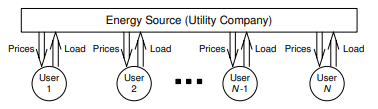
\includegraphics[width=0.8\textwidth]{img/teoria/dsm1.png}
  \caption{Estrategia de \gls{dsm} basada en interacciones individuales de cada consumidor con la compañía \cite{pricing}}
  \label{fig:dsm1}
\end{figure}

Con este proceso, el consumidor como puede saber en tiempo real la tarifa a la que está consumiendo energía, puede trasladar su propia carga desde las horas donde el precio es más alto (horas pico) a las de precio menor (horas valle). Esta gestión produce por tanto, menores picos de demanda y contribuyendo a la bajada de los precios. \cite{dsm} \cite{pricing}

\vspace{3mm}

No obstante, el diseño de un programa \gls{dsm} ideal en el contexto de las \gls{sg}s debería permitir también las interacciones entre los mismos prosumidores dentro de una zona residencial o microgrid. Estas interacciones generalmente se automatizan a través de equipos dedicados a una comunicación digital bidireccional. Como se aprecia en la Figura \ref{fig:dsm2}, este proceso tiene como fin conducir a una coordinación de las acciones respectivas a las cargas de un área determinada. 

\vspace{3mm}

Por tanto, en este caso la monitorización de las cargas totales para todos los nodos participantes en un instante determinado aportará la información necesaria sobre la relación entre la potencia pico y promedio (del inglés \gls{par}) y contribuirá a la fijación del precio unitario para ese mismo instante. \cite{pricing} 

\begin{figure}[h!]
  \centering
  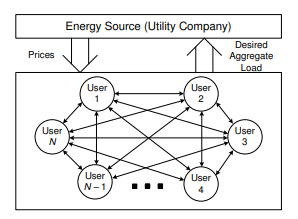
\includegraphics[width=0.65\textwidth]{img/teoria/dsm2.png}
  \caption{Estrategia de \gls{dsm} para smart grids basada en interacciones entre los usuarios y la compañía \cite{pricing}}
  \label{fig:dsm2}
\end{figure}


%%%%%%%%%%%%%%%%%%%%%%%%%%%%%%%%%%%%%%%%%%%%%%%%%%%%%%%%%%%%%%%%%%
\subsection{Estructura de una Smart Grid}

Una \gls{sg} está constituida por múltiples elementos diferentes como se puede visualizar en la Figura \ref{fig:estructura_sg}. Cada uno de ellos está dedicado a uno de los procesos principales, que se pueden dividir en generación, distribución y consumo. \cite{smartgrid_overview}

\begin{figure}[h!]
  \centering
  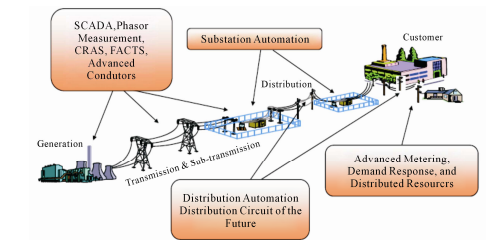
\includegraphics[width=1\textwidth]{img/teoria/estructura_sg.png}
  \caption{Estructura de componentes de una \gls{sg} \cite{smartgrid_overview}}
  \label{fig:estructura_sg}
\end{figure}

\subsubsection{Generación}

Como ya se introducía en la Sección \ref{sec:prosu}, dentro de una \gls{sg}, el prosumidor se trata de la figura que potencia principalmente el uso de energías renovables, las cuales pueden ser obtenidas por ejemplo a partir de generadores térmicos fotovoltaicos (del inglés \gls{pvt}) o de turbinas eólicas. Para posibilitar posteriormente el uso de la energía generada, esta debe ser convertida y acondicionada mediante dispositivos dedicados, como son unidades combinadas de calor (del inglés \gls{chp}) o de conversión a gas (del inglés \gls{p2g}). \cite{transactive}

\vspace{3mm}

Las unidades \gls{chp} \cite{chp} llevan a cabo un aprovechamiento del calor residual que deriva del proceso de generación de electricidad. Se emplean como respaldo eléctrico, ya que se componen de sistemas de almacenamiento de energía térmica (del inglés \gls{tes}) para poder separar la producción y el uso del calor y la energía. Luego, este calor almacenado se puede emplear en aplicaciones térmicas como la calefacción u otros procesos industriales. Es por ello que las unidades \gls{chp} mejoran la eficiencia del sistema energético, contribuyendo a un uso mucho más eficaz de los recursos y a una reducción de las pérdidas que se producen en la transmisión. En la Figura \ref{fig:chp} se representa a modo esquemático el funcionamiento de una unidad \gls{chp}. \cite{chp2}

\begin{figure}[h!]
  \centering
  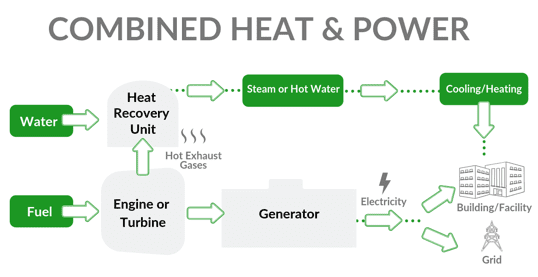
\includegraphics[width=0.9\textwidth]{img/teoria/chp.png}
  \caption{Esquema de funcionamiento de una unidad \gls{chp} \cite{chp}}
  \label{fig:chp}
\end{figure}

Además del \gls{tes}, utilizado para almacenar el calor producido, una unidad \gls{chp} también se constituye de un motor acoplado a un generador eléctrico para llevar a cabo el proceso de generación de electricidad y calor. Como se puede apreciar en la Figura \ref{fig:chp2}, todas las operaciones de la unidad y las interacciones que se producen entre módulos se coordinan desde el gestor de operaciones para que se produzca un correcto funcionamiento.

\begin{figure}[h!]
  \centering
  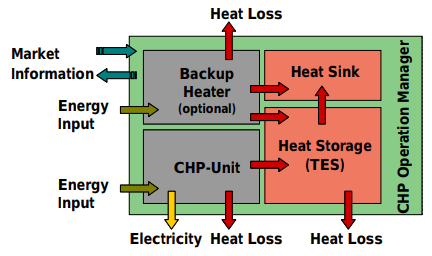
\includegraphics[width=0.65\textwidth]{img/teoria/chp2.png}
  \caption{Gestión de operaciones en una unidad \gls{chp} \cite{chp2}}
  \label{fig:chp2}
\end{figure}

Por otro lado, la unidad \gls{p2g}, mencionada anteriormente, se encarga de la conversión de la electricidad en gases sintéticos, como son el hidrógeno o el metano. Es de gran importancia, ya que este tipo de gases son más fácil de transportar y almacenar que la electricidad, por lo que se simplifica la gestión energética. \cite{transactive}

\vspace{3mm}

Como se puede apreciar en la Figura \ref{fig:p2g}, el objetivo del \gls{p2g} se basa en descomponer el agua mediante un proceso de electrólisis a partir de electricidad proveniente de fuentes renovables. Después, el hidrógeno que se produce se puede utilizar directamente o procesarlo de forma adicional en metano. 

\begin{figure}[h!]
  \centering
  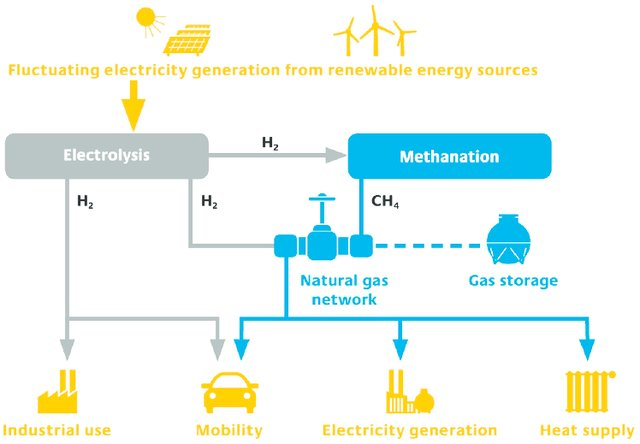
\includegraphics[width=0.85\textwidth]{img/teoria/p2g.jpg}
  \caption{Representación del proceso \gls{p2g} \cite{p2g}}
  \label{fig:p2g}
\end{figure}

Dentro del contexto de la generación de energía también es importante destacar algunos equipos, como son los sistemas de control y adquisición de datos (del inglés \gls{scada}) \cite{scada}. Estos pueden ser instalados en generadores, como son paneles solares fotovoltaicos o turbinas eólicas, consiguiendo una monitorización remota de los mismos. Mediante la información recopilada a tiempo real permiten conocer los niveles de generación y establecer una predicción de la disponibilidad energética que habrá en el sistema o en un área determinada del mismo.

\vspace{3mm}

\subsubsection{Distribución}

Un dispositivo importante en el campo de la distribución energética es la Unidad de Medición de Fasores (del inglés \gls{pmu}). Se emplea para medir con una alta precisión los fasores de tensión y corriente en la red eléctrica, proporcionando información relevante sobre las magnitudes y fases de las ondas sinusoidales. 

\vspace{3mm}

También, es empleado en los generadores y debe contar con una alta tasa de muestreo para capturar eventos transitorios o cambios rápidos en la red. En otros términos, debe tener la capacidad de identificar o detectar a tiempo real posibles anomalías que se puedan dar en la distribución y por ello, se trata de un componente imprescindible para comprobar y garantizar la estabilidad de la \gls{sg}. %BIB

\vspace{3mm}

La confiabilidad y la seguridad de la red también reside en los Sistemas de Transmisión de Corriente Alterna Flexibles (del inglés \gls{facts}) \cite{facts} \cite{facts3}. Estos vienen dados por la necesidad de superar las limitaciones técnicas introducidas por las redes eléctricas, como son las térmicas o las respectivas al voltaje. En otros términos, incrementan la potencia transmitida y aportan flexibilidad al permitir modificar de forma dinámica los parámetros eléctricos ante cambios en la configuración de la red. 

\vspace{3mm}

Los \gls{facts} incluyen todos los elementos electrónicos basados en tecnología de alta potencia y que son empleados dentro de una \gls{sg} para la transferencia de energía de CA y el control de la potencia reactiva. También, realizan tareas de reducción de impedancia en las líneas de transmisión y de optimización del factor de potencia y pueden actuar tanto a nivel individual como de forma coordinada con otros controladores.

\vspace{3mm}

La primera generación de \gls{facts} emplea interruptores controlados por tiristores, mientras que la segunda tiene como base convertidores estáticos de conmutación. En la Tabla \ref{tab:facts} se visualizan las tecnologías \gls{facts} más relevantes. \cite{facts2} \cite{facts3}

\begin{table}[!h]
    \centering
    \resizebox{\textwidth}{!}{
    \begin{tabular}{| c | c | m{6cm} |}
    \hline
    \rowcolor[HTML]{EFEFEF}
    Generación & Tipo & \multicolumn{1}{c|}{Descripción} \\ \hline
    \multirow{2}{*}{1º} 

    & \gls{tcsc} & Controla el flujo de potencia tanto reactiva como activa por la línea de transmisión mediante el ajuste de impedancia en serie y amortigua las oscilaciones.
    
    \\ \cline{2-3}

    & \gls{svc} & Absorbe o suministra potencia reactiva según las necesidades de una línea de transmisión a través de la variación de la susceptancia en paralelo. Ayuda a mantener el voltaje estable en la red y proveen un aumento de la capacidad de transferencia de energía.

    \\ \hline
    \multirow{4}{*}{2º} 
    
    & \gls{statcom} & Compensa la potencia reactiva al igual que el \gls{svc}, pero en este caso empleando electrónica de potencia para proporcionar una respuesta más rápida.

    \\ \cline{2-3} 

    & \gls{upfc} & Combina las funciones de un \gls{tcsc} y un \gls{svc}, teniendo la capacidad de controlar en una línea de transmisión tanto la impedancia en serie como la susceptancia en paralelo.

    \\ \cline{2-3} 

    & \gls{sssc} & Modifica dinámicamente la impedancia y es capaz de controlar la fase y la amplitud de la tensión en la línea.

    \\ \cline{2-3} 

    & \gls{ipfc} & Conecta varias líneas de transmisión en paralelo. No obstante, modula la impedancia y la fase de la tensión de cada línea de transmisión de forma independiente, lo que permite operar sobre el flujo de potencia de una forma controlada. Mejora la capacidad de transmisión y reduce las pérdidas energéticas. 
    
    \\ \hline
    \end{tabular}
    }
    \caption{Tecnologías FACTS de 1ª y 2ª generación}
    \label{tab:facts}
\end{table}

Poniendo el enfoque en la garantía de estabilidad de una \gls{sg}, uno de los sistemas más importantes de los expuestos en la Tabla \ref{tab:facts} es el \gls{svc} \cite{facts}. Los compensadores estáticos son capaces de detectar grandes caídas de tensión resultantes a la producción de un cortocircuito o a la pérdida de líneas de transisión en un área de la red. Esto es importante, ya que una detección rápida de una avería permite restaurar en un corto período de tiempo la tensión del área afectada sin que el problema escale a otras partes de la red. 

\vspace{3mm}

En otros términos, aísla este área del resto de la red eléctrica. Además, el \gls{svc} asegura que el proceso de restauración se produzca paulatinamente para que los efectos producidos por el cortocircuito sean prácticamente imperceptibles en los puntos de carga del área afectada. En la Figura \ref{fig:svc} se puede apreciar un ejemplo de instalación de un \gls{svc} en el municipio noruego Sylling y se encuentra conectada a un sistema de 420 kV.

\begin{figure}[h!]
  \centering
  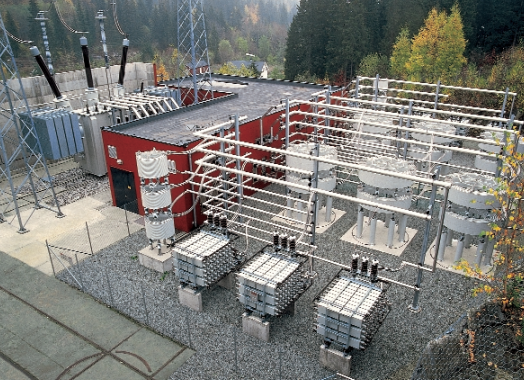
\includegraphics[width=0.7\textwidth]{img/teoria/svc.png}
  \caption{Instalación de un \gls{svc} en Sylling (Noruega) \cite{facts}}
  \label{fig:svc}
\end{figure}

Siguiendo en el ámbito de la distribución energética, es importante también exponer las tecnologías enfocadas a la transmisión de electricidad a larga distancia, como son las Corriente Continua de Alto Voltaje (del ingles \gls{hvdc}) \cite{hvdc}. Como su nombre indica, utilizan corriente continua para ello, lo que minimiza las pérdidas en el proceso de transmisión respecto al caso de la Corriente Alterna de Alto Voltaje (del ingles \gls{hvac}), además de permitir portar mucha más potencia. 

\vspace{3mm}

Esto es fundamental cuando se pretende integrar al sistema global fuentes de energía ubicadas en áreas remotas, sobre todo dentro del contexto de las \gls{sg}s. Generalmente, las fuentes de energías renovables, como pueden ser la solar o la eólica, se encuentran alejadas de los puntos geográficos con mayor demanda y se requiere una respuesta rápida ante cambios de carga para mantener la estabilidad del sistema. 

\vspace{3mm}

Es decir, cuando se transmiten grandes cantidades de potencia a largas distancias con líneas de \gls{hvac}, se generan ángulos eléctricos entre los voltajes y las corrientes en la línea muy grandes que pueden producir oscilaciones descontroladas y por tanto, desencadenar inestabilidades que llegaráin a escalar a lo largo del sistema. 

\vspace{3mm}

Por ello, las tecnologías \gls{hvdc} simplifican la interconexión entre microrredes y permiten una mayor integración de sistemas dedicados al almacenamiento energético para facilitar la gestión de los recursos disponibles. Como desventaja, se encuentra el alto coste que supone su implementación, ya que al final solamente se puede emplear en el caso de aplicaciones punto a punto.

\vspace{3mm}

En la Figura \ref{fig:hvdc} se muestra como ejemplo una infraestructura de transmisión de energía eólica a larga distancia. Esta energía proviene de una fuente remota y se transporta a través del medio marino para llegar hasta los usuarios. Como se puede apreciar, es necesario implementar estaciones de conversión de alto voltaje de corriente alterna a continua y viceversa en los extremos de las líneas \gls{hvdc}.

\begin{figure}[h!]
  \centering
  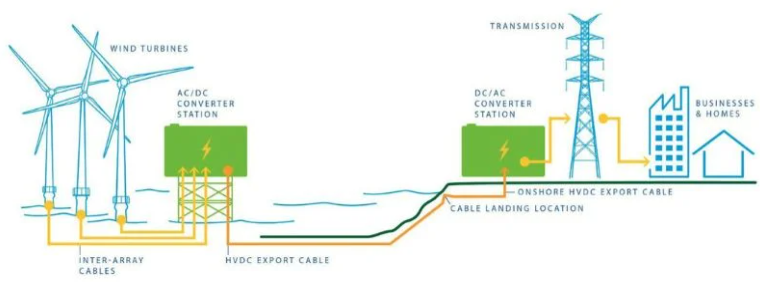
\includegraphics[width=0.9\textwidth]{img/teoria/hvdc.png}
  \caption{Representación de un sistema de transmisión de energía eólica con líneas \gls{hvdc} \cite{hvdc2}}
  \label{fig:hvdc}
\end{figure}

\subsubsection{Consumo}
\label{sec:consumo}

Entrando en detalle en las ubicaciones finales del sistema y por tanto, en el proceso de consumo, es imprescindible conocer la cantidad de energía demandada por los clientes que pertenecen a una \gls{sg}. La instalación de sensores o medidores inteligentes (del ingles \textit{smart meters}) en las viviendas posibilitan el registro constante de datos respectivos al consumo de energía, niveles de voltaje, corriente y factor de potencia. Estos son almacenados, analizados y procesados por las distribuidoras de energía para obtener a partir de los mismos la información necesaria sobre el comportamiento de los usuarios. \cite{stab}

\vspace{3mm}

Como se había introducido en el Apartado \ref{sec:smartgrids} el proceso de adquisición de datos por parte de los usuarios se trata de uno de los pilares más relevantes de cara a la optimización energética del sistema. Los objetivos principales que se pretenden con este proceso se engloban en la reducción del consumo, la optimización de la distribución y la maximización del beneficio. Respecto a este último, las compañías energéticas a partir de su base de clientes estudian las estrategias de categorización de los mismos para definir el sistema de fijación de precios dinámicos. \cite{stab}

\vspace{3mm}

No obstante, la gestión de los sensores finales en las \gls{sg}s se caracteriza por su alta complejidad, debido a los grandes volúmenes de datos a manejar. Se requiere un procesamiento eficiente a tiempo real para analizar datos capturados de múltiples fuentes con el fin de evitar latencias o bloqueos en el sistema. Es por ello que se dificulta el empleo de herramientas convencionales de gestión de bases de datos y se requiere una solución más avanzada mediante la aplicación de tecnologías enfocadas al \textit{Big Data}. Se profundizará más sobre ello en la Sección \ref{sec:bigdata}.

\vspace{1mm}

%%%%%%%%%%%%%%%%%%%%%%%%%%%%%%%%%%%%%%%%%%%%%%%%%%%%%%%%%%%%%%%%%%
\subsection{Protocolos}
% a) Green-RPL
% (b) Local positive degree coupling
% (c) IEEE 802.11s
% (d) Web Of Energy
% (e) Dynamic Barrier Coverage
% (f) IEC61850
% (g) Wind-driven bacterian foraging algorithm
% (h) Data Slicing
% (i) TSUBE energy trading algorithm
% (j) Stochastic Geometry
% (k) Rectangular quadrature amplitude modulation
% (l) Policy-based group authentication algorithm
% (m) Mapping interface integration COIIoT
% (n) Nash Equilibrium (NE) and the Bayesian NE
% (o) Wireless sensor network protocol
% (p) Algorithmic Approach


%Green-RPL, Local positive degree coupling, IEEE 802.11s, Web Of Energy, Dynamic Barrier Coverage, IEC61850, Wind-driven bacterial foraging algorithm, Data Slicing, TSUBE energy trading algorithm, Stochastic Geometry, Rectangular quadrature amplitude modulation, Policy-based group authentication algorithm, Mapping interface integration COIIoT, Nash Equilibrium (NE) and the Bayesian NE, Wireless sensor network protocol and Algorithmic Approac

%ver tabla https://electrical-engineering-portal.com/smart-grid-deployment-what-weve-done-so-far


\vspace{1mm}

%%%%%%%%%%%%%%%%%%%%%%%%%%%%%%%%%%%%%%%%%%%%%%%%%%%%%%%%%%%%%%%%%%
\subsection{Topología de red}

% Smart Grid Network Topology
% (a) Neighborhood Area Networks (NAN)
% (b) Software-Defined Networks (SDN)
% (c) Interdependent Networks (IN)
% (d) Field Area Networks (FAN)
% (e) Wireless Sensor Networks (WSN)
% (f) Not Defined
%NAN, FAN AND THE SDN are widely used network topology



\vspace{1mm}

%%%%%%%%%%%%%%%%%%%%%%%%%%%%%%%%%%%%%%%%%%%%%%%%%%%%%%%%%%%%%%%%%%
\subsection{Seguridad en Smart grids}
\label{sec:seg}
 
Como se ha introducido en la Sección referente a la figura del prosumidor (ver Sección \ref{sec:prosu}), el \gls{dso} tiene la capacidad de operar ante problemas y fallos en la red tomando decisiones y dando una respuesta rápida. En determinados casos las incidencias se pueden dar por la configuración del propio sistema, si esta no se realiza de forma correcta y eficiente. No obstante, también es preciso contemplar la posibilidad de ataques externos que atenten contra el sistema de la \gls{sg}.

\vspace{3mm}

Uno de los ataques más peligrosos en este ámbito es el de Inyección de Datos Falsos (del inglés \gls{fdi}) \cite{baddata} y, como su nombre determina, se basa en la inyección de paquetes maliciosos en la red con el fin de bloquear los servicios de la misma y conseguir la autorización para realizar operaciones restringidas. El proceso se puede realizar actuando directamente a través de los sensores finales (\textit{smart meters}) o secuestrando el canal de comunicación. Algunas técnicas empleadas por los atacantes son las siguientes \cite{baddata}:

\begin{itemize}
  \item Fallo del dispositivo: Se aplica un ataque de Denegación de Servicio (del inglés \gls{ddos}) a los sensores. Cabe destacar que generalmente los sensores que se encuentran en las ubicaciones finales tienen una capacidad limitada de conexión que derivaría en grandes latencias en la comunicación de datos con el resto de entidades de la red. En este momento el atacante se encarga de suplantar al host en cuestión para enviar los paquetes falsos en su nombre.
  \item \textit{Cracking}: Se descifran las contraseñas para obtener acceso a los equipos mediante ingeniería social o fuerza bruta. De la misma forma que el anterior, la limitación de los recursos computacionales de los sensores provoca que no existan mecanismos de contraseñas lo suficientemente seguros. Además, la mayoría de ellos emplean como protocolos de comunicación Modbus/TCP o DNP 3.0/TCP, los cuales implementan una transmisión de texto en formato plano y sin cifrado. Por ello, un atacante puede tener la posibilidad de monitorear y capturar el tráfico si consigue acceso.
  \item Envenenamiento de tablas \gls{arp} o \textit{\gls{arp} Spoofing} \cite{arp}: Consiste en enviar mensajes falsos \gls{arp} para monitorizar el tráfico y capturar o alterar los paquetes que se están transmitiendo por la red. 
\end{itemize}

Teniendo esto en cuenta, es imprescindible definir los mecanismos de detección y mitigación a emplear para evitar que se produzcan ataques \gls{fdi} \cite{baddata}:

\begin{itemize}
  \item Mecanismo de autenticación estrictos: Los datos que se suministran al \gls{dso} o a otras entidades de control de la \gls{sg} deben de ser autenticados para comprobar su confiabilidad. Para ello, se emplean por ejemplo, marcas de tiempo para evitar ataques de repetición y protocolos de seguridad como \gls{tls} o \gls{ssl}, además de \gls{sha} y \gls{hmac}.
  \item Gestión dinámica de claves: Se actualizan las claves con una determinada frecuencia para incrementar la seguridad de los estándares \gls{ieee} 802.11s y evitar ataques \gls{ddos}.
  \item Empleo del protocolo \gls{send} \cite{send}: Para evitar los ataques de \textit{\gls{arp} Spoofing} se emplean pares de claves \gls{rsa} para poder garantizar en el proceso de enrutamiento que los mensajes que tienen como origen un determinado host pertenecen al mismo.
\end{itemize}



%a partir del 3.4 del AI-based FDI Countermeasure for IoE Smart Grids

%%%Energy Big Data: A Survey pag 10 figura















\vspace{1mm}

%%%%%%%%%%%%%%%%%%%%%%%%%%%%%%%%%%%%%%%%%%%%%%%%%%%%%%%%%%%%%%%%%%
\subsection{Estándares y regulación en smart grids}

%estándares smart grids -> cite OUTLOOK FOR INCREASED ADOPTION OF SMART GRID TECHNOLOGIES IN ADB ENERGY SECTOR OPERATIONS

% International Technical Standards for Smart Grids (Smart Grid Codes)
% Grid code development and implementation is a critical area in smart grid implementation. It has to be 
% aligned with the standards being used in respective countries and international standards. This is an 
% important first step in smart grid implementation. Some of the international standards are as follows.
% (i) IEEE1547 Family of Standards. IEEE 1547 family of standards deals with smart grid components 
% involving distributed resources interconnection. Released in 2003, this provides the basis and 
% sets the standards for the integration of distributed energy generation by detailing requirements 
% related to interconnection performance, operation, testing, safety, and maintenance.
% (ii) IEEE 2030 Family of Standards. The  IEEE Standard 2030–2011’s “Guide for Smart Grid 
% Interoperability of Energy Technology and Information Technology Operation with the 
% Electric Power System, and End-Use Applications and Loads” is the root standard of the 2030 
% series. This standard provides alternative approaches and best practices for achieving smart 
% grid interoperability.
% (iii) IEC Family of Standards. IEC has identified over 100 standards relevant to smart grids. The 
% following are core standards: (i) IEC/TR 62357: Service Oriented Architecture; (ii) IEC/61970: 
% Common Information Model/Energy Management; (iii) IEC 61850: Power Utility Automation; 
% (iv) ICC/61968: Common Information Model/Distribution Management; IEC 62351: Security; 
% (v) IEC 62056: Data Exchange for Meter Reading, Tariff and Load Control; and (vi) IEC 61508: 
% Functional Safety of Electrical, Electronic, Programmable Electronic Safety Related Systems.


\vspace{1mm}

%%%%%%%%%%%%%%%%%%%%%%%%%%%%%%%%%%%%%%%%%%%%%%%%%%%%%%%%%%%%%%%%%%
\subsection{Beneficios ambientales}

%Las smart grid son un concepto estratégico clave en la transición energética, ya que suponen un gran paso hacia un mundo descarbonizado. Mediante la digitalización de las redes eléctricas inteligentes se puede conseguir un sistema más eficiente, sostenible, con bajas pérdidas y con altos niveles de calidad en el suministro. Con la implementación de este circuito inteligente no solo se conseguiría una mayor eficiencia energética y ahorro, sino que también tendría múltiples beneficios medioambientales, económicos y sociales.


% La eficiencia energética que se pueden conseguir con las smart grid también tiene beneficios directos sobre el medio ambiente, como por ejemplo: 

% Permiten el desarrollo de ciudades sostenibles.
% Pueden integrarse en el sistema de fuentes renovables.
% Facilitan la movilidad eléctrica, proporcionando puntos de carga para vehículos eléctricos.
% Reducen las emisiones globales de CO2.
% Contribuye a la descarbonización de la generación eléctrica. 


\vspace{1mm}

%%%%%%%%%%%%%%%%%%%%%%%%%%%%%%%%%%%%%%%%%%%%%%%%%%%%%%%%%%%%%%%%%%
\subsection{Situación en España}

En el caso de España, nuestro país ocupa el quinto lugar en el mercado eléctrico europeo, solamente por detrás de Alemania, Francia, Reino Unido e Italia. 

%buscar datos españa

Además, en los último años ha crecido en consideración 

y está creciendo rápidamente. La demanda eléctrica estimada para el año 2001 fue de 210.4 mil millones de kilovatios-hora (bkwh), un aumento del 5% respecto al año 2000. Se estima que la demanda eléctrica de España aumentará un 30% para el año 2010.

% Para hacer frente al aumento de la demanda eléctrica en España, las empresas de servicios públicos nacionales han invertido en capacidad de generación y distribución. Red Eléctrica de España (REE), por ejemplo, invirtió considerablemente en la red en 2001, destinando 78.4 millones de euros a la expansión de la red eléctrica. En octubre de 2001, REE también anunció planes para invertir entre 60.2 y 72.2 millones de euros para mejorar la conexión eléctrica con Francia. Las tres mayores compañías eléctricas de España: Endesa, Iberdrola y Unión Fenosa, han dedicado 34 mil millones de euros en inversiones desde agosto de 2001 hasta 2005, gran parte de ellas en América Latina y otros países europeos, pero incluyendo aún así 8 mil millones de euros para nuevas plantas generadoras en España.

% Endesa está construyendo actualmente una planta de turbina de gas de ciclo combinado (CCGT) de 400 MW en Huelva, además de otras dos CCGT de gas de 400 MW que la empresa ya tiene en construcción en Barcelona y Tarragona. Endesa completó recientemente la construcción de una planta con 8,000 MW en Cádiz. Unión Fenosa planea agregar 5,000 MW de nueva capacidad para 2005, principalmente en España, de los cuales 2,800 MW serían de gas natural. Piemsa, una filial de Petronor, planea construir un complejo de gasificación integrada de ciclo combinado (IGCC) de 800 MW en una refinería cerca de Bilbao que utilizará productos pesados de la refinería. La planta será una de las más grandes y avanzadas de su tipo en el mundo.


%https://www.smartgridsinfo.es/2020/01/23/6-congreso-smart-grids-refuerza-consolida-redes-electricas-inteligentes-politica-energetica-espana

\cite{spain}


\begin{figure}[h!]
  \centering
  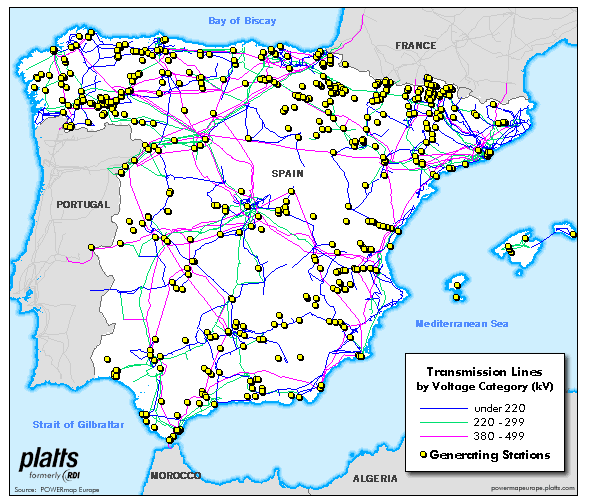
\includegraphics[width=0.8\textwidth]{img/teoria/spain.png}
  \caption{Red nacional de transmisión energética \cite{spain}}
  \label{fig:spain}
\end{figure}







\vspace{1mm}

%%%%%%%%%%%%%%%%%%%%%%%%%%%%%%%%%%%%%%%%%%%%%%%%%%%%%%%%%%%%%%%%%%
\subsection{Desafíos futuros de las smart grids}

%%%%\cite{overview} Smart Grid: An Overview

% The Key Challenges for Smart Grids 
%  Strengthening the grid—ensuring that there is sufficient transmission capacity to interconnect energy resources, especially renewable resources; 
%  Moving offshore—developing the most efficient connections for offshore wind farms and for other marine 
% technologies; 
%  Developing decentralized architectures—enabling smalller scale electricity supply systems to operate harmoniously with the total system; 
%  Communications—delivering the communications infrastructure to allow potentially millions of parties to 
% operate and trade in the single market; 
%  Active demand side—enabling all consumers, with or 
% without their own generation, to play an active role in 
% the operation of the system; 
%  Integrating intermittent generation—finding the best 
% ways of integrating intermittent generation including 
% residential microgeneration; 
%  Enhanced intelligence of generation, demand and most 
% notably in the grid; 
%  Preparing for electric vehicles—whereas Smart Grids 
% must accommodate the needs of all consumers, electric vehicles are particularly emphasized due to their 
% mobile and highly dispersed character and possible 
% massive deployment in the next years, what would 
% yield a major challenge for the future electricity networks [2]. 




%%%%cite us


%4.0 Desafíos para la implementación
% Entre los desafíos importantes que enfrenta el desarrollo de una red inteligente se encuentran el costo de
% de implementación de una red inteligente, con estimaciones solo para la medición avanzada de la empresa eléctrica
% de capacidad que asciende a $27 mil millones, y las regulaciones que permiten la recuperación de dicha
% inversiones. Para tener una perspectiva, Brattle Group estima que podría tomar tanto como
% 1,5 billones de dólares para actualizar la red para 2030 (Chupka et al. 2008). Garantizar la interoperabilidad % de estándares de redes inteligentes es otro obstáculo que los reguladores estatales y federales deberán superar.
% Las principales barreras técnicas incluyen el desarrollo de sistemas de almacenamiento económicos; estos sistemas de almacenamiento
% puede ayudar a resolver otros desafíos técnicos, como la integración de energía renovable distribuida
% de fuentes con la red, abordando problemas de calidad de energía que de otro modo exacerbarían la
% de situación y mejorar la utilización de los activos. Sin red inteligente, altas penetraciones de variables
% de recursos renovables (por ejemplo, eólicos o solares) pueden volverse cada vez más difíciles y costosos de obtener.
% logran con el tiempo a medida que penetran a niveles altos debido a la mayor necesidad de coordinar estos
% de recursos con generación despachable (p. ej., ciclo combinado de gas natural) y demanda.
% Otro desafío al que se enfrenta una red inteligente es la incertidumbre sobre el camino que seguirá su desarrollo.
% se hace cargo del tiempo con la tecnología cambiante, los cambios en las combinaciones de energía y la política energética.
% Intentar legislar o regular el desarrollo de una red inteligente o sus tecnologías relacionadas puede
% disminuyen gravemente los beneficios del mercado energético virtual, flexible y transparente al que se esfuerza.
% Para proveer. Por el contrario, con la red energética de todo el país potencialmente en riesgo, algunos pueden ver
% la introducción de una red inteligente en los Estados Unidos es demasiado importante para permitir el laissez-faire
% evolución. Por lo tanto, el desafío del desarrollo se convierte en una cuestión de proporcionar servicios flexibles
% de regulación que aprovecha la tecnología deseada y en desarrollo a través de objetivos dirigidos y
% de políticas respaldadas por casos de negocios que promueven un resultado económico positivo. Estos y otros
% de desafíos se analiza en las siguientes secciones


\subsubsection{Retos técnicos}

% There are a variety of technical challenges facing a smart grid, some of the greatest being 
% developing, implementing, and deploying the array of different technologies required to 
% enable both sides of the meter to communicate in a cost-effective way. One of the most 
% important developments facing a smart grid is AMI technology. These devices help 
% coordinate consumer equipment, as well as receive market signals and adjust household 
% consumption based on a combination of this data and consumer preferences. However, 
% alternatives to such AMI systems do exist. For example, market information such as prices 
% and grid conditions can be decoupled from communication of energy consumption. Thus, 
% the meter can be separate while pricing signals and the like can be transmitted via other public 
% communication mechanisms such as phone, internet, cable, and wireless radio. A decoupled 
% situation can make sense for commercial buildings and industrial uses where energy savings 
% can be significant, while a more traditional bundled AMI package may be more desirable for 
% residential consumers due to its “all-in-one” and “plug-and-play” aspects. Implementing 
% price- and consumption-bundled AMI technology has been estimated to cost as much as 
% $27 billion (Kuhn 2008) and will require very aggressive deployment to meet desired market 
% penetration levels in the near future. Failure to successfully deploy technology that captures 
% bi-directional power flow rather than net consumed energy, as well as dynamic pricing 
% support, such as AMI technology or others, will keep the two sides of the market from 
% properly communicating, and a smart grid will not function as desired regardless of other
% successful technical deployments, such as distributed generation, demand-response measures, 
% or automated distribution schemes. Without real-time demand-response signals being 
% promptly communicated and quickly addressed by consumers, the power system will not 
% be flexible enough to provide the market transparency or the price signals required for a 
% functioning energy market (FERC 2006a). Further, AMI billing techniques and the machines 
% themselves may require regional customization reducing potential economies of scale in 
% production and deployment. Regional customization may be required because of differences 
% in consumer preferences, aggressiveness of service providers, state and local regulations, and 
% the speed with which smart grid structures and technology change over time. Not all regions 
% are likely to respond identically and may have different needs.
% Another significant technical consideration is the impact of high levels of new technology 
% penetration on existing grid infrastructure. Implementing new improvements into the grid, 
% including smart-grid technologies, is pivotal to increasing efficient operations, as the operating 
% efficiency gains from familiar technologies have begun to plateau (DOE/EIA 2007a). In 
% addition, a NERC survey recently ranked the number one challenge to grid reliability as 
% “aging infrastructure and limited new construction.” How this aging infrastructure will 
% function when combined with new “smart” technology remains to be seen, particularly with 
% regard to solar, wind, and other forms of distributed generation (NERC 2007). Adding large 
% amounts of variable and distributed generation, for example, requires a fundamental 
% reworking of how the delivery system is managed, power quality is monitored, faults are 
% detected, and maintenance is handled (Pai 2002). This problem is compounded when 
% PHEVs and EVs are considered, potentially making each vehicle its own DG resource and 
% requiring supporting infrastructure to draw, generate, and price power transactions. 
% However, these technologies themselves face several technical challenges. Cost-effective 
% battery technology continues to be a challenge for PHEVs and EVs and local wind and solar 
% resources. Issues such as discharge, battery life, size and weight are all serious considerations. 
% Additionally, incorporating battery power storage into current automobile frames will require 
% manufacturing adjustments; including systems to monitor the status of the battery (including 
% battery charge and temperature) as well as structural design changes to accommodate the 
% battery itself.

% A smart grid is needed at the distribution level to manage voltage levels, reactive power, 
% potential reverse power flows, and power conditioning, all critical to running grid-connected 
% DG systems, particularly with high penetrations of solar and wind power and PHEVs. 
% Advanced voltage regulation, fault-detection, and system-protection practices need to be 
% rethought as an increasing number of DG resources become available. This may require new 
% equipment to identify and isolate DG resources in the event of a fault occurrence (Driesen 
% and Belmans 2006). Another consideration for power-generation systems, distributed or 
% otherwise, is power quality. Customers and the utilities that serve them lack standards for 
% classifying varying qualities of power. Because customers have different power quality 
% requirements (e.g., willingness to accept outages of varying durations, and load sensitivity to 
% power harmonics) and with the increasing availability of DG resources to produce power 
% locally, there may be smaller sub-markets for power that would be better served if such 
% differentiated power standards existed.
% Designing and retrofitting household appliances, such as washers, dryers, and water heaters 
% with technology to communicate and respond to market signals and user preferences via 
% home automation technology will be a significant challenge. Substantial investment will be 
% required to implement user-friendly communication equipment which ensures that data
% storage and transmissions are tamper proof, reliable, and do not corrupt or break down over 
% the lifetime of an appliance. Devices that communicate wirelessly with their facility energymanagement systems must broadcast powerful-enough signals, or other technical barriers to 
% effective communication must be resolved. For example, a washer/dryer located in a house’s 
% basement attempting to communicate with an energy-management system on the far side of 
% the building will require a stronger signal than a closer device on the ground floor. Therefore 
% communication equipment may need a flexible and dynamic range of broadcast strengths. 
% Finally, aggregating and sharing system data involves its own concerns; for example, providing 
% infrastructure to communicate wide-area measurement data across the grid requires agreement 
% by the stakeholders on the information network architecture, the supported functions, data 
% exchange interface definitions, and legal conditions for granting use of the data.

\subsubsection{Retos económicos}

% The business case for a smart grid needs to be firmly established for deployment decisions to 
% progress. In many situations, individual applications may not be cost effective in isolation, 
% but where common hardware and information network infrastructure can be leveraged to 
% accomplish a number of objectives, the value proposition can become compelling. The 
% business challenge is to prove that out with field deployments. Smart grid investments often 
% require large upfront costs relative to their benefits. However, future benefits may come at 
% small incremental costs. Utilities and regulators may need to look at full system life cycle 
% costs and benefits in order to fully justify added investments. Some of the benefits may come 
% in the form of societal benefits which will need to be clearly understood and evaluated. 
% Payback periods may be longer than stakeholders would like. The service providers, regulators, 
% and ultimately ratepayers are going to have to believe it before such substantial investments 
% are made.
% Since the technology and value propositions are emerging, utility companies may be reluctant 
% to expend the significant amount of capital required to move toward a smart grid, especially 
% because expected cost-recovery timelines are only theoretical and have no precedent. 
% Currently, regulated utilities and their flat-rate customers have no risk or reward signal. 
% Regulation makes it difficult for them to raise rates and recover costs, and makes them 
% reluctant to change. Moreover, transmission-planning difficulties may or may not offset 
% revenue losses incurred from reduced transmission; with uncertainty about market penetration 
% of DG these effects can be difficult to model. Without effective cost recovery mechanisms in 
% place, increased market penetration of DG will translate into lost demand for utilities. The 
% uncertainty about market penetration is increased when utilities start to consider the time and 
% cost of training a new smart-grid-skilled labor force (NERC 2007). Thus, utilities seeking to 
% balance costs and operating efficiency will seek to increase asset utilization through the 
% implementation of demand response measures and AMI technology, as opposed to expensive 
% infrastructure upgrades. Further, as more and more devices become “web enabled” and move 
% toward becoming fully “smart” devices, the inclusion of electronics in these devices, as well as 
% the development and maintenance of this hardware and its respective software, will require 
% manufacturers to reevaluate these devices’ life-cycle costs. A smart grid will require service 
% providers to operate in new ways and be willing to take reasonable risks for reasonable 
% rewards. Regulators will need to design rules such that customers who do not change are not 
% worse off, but that businesses can pursue advantageous arrangements between participating 
% suppliers and consumers. Aside from making a strong analytical business case with existing distribution models, the first 
% few successful deployments of these new “smart” technologies will be pivotal to ensuring deep 
% market penetration. Not all of these technologies are necessarily complementary. For 
% example, when metering residential customers, drive-by and walk-by meters (AMR) are 
% considered a competing technology and currently are out-shipping AMI products. Other 
% than the more-convenient data gathering over traditional meters, AMR meters offer very few 
% to none of the benefits and functions necessary to enable residential customers to 
% meaningfully participate in a smart grid. However, implementing smart-grid technologies is 
% daunting; the cost to implement AMI technology alone has been forecast between $19 and 
% $27 billion (Kuhn 2008). Customers desire good value for the investments reflected in their 
% power bills and they may want more options to manage their energy usage and bills, especially 
% during a rate increase.

% While utilities must be able to recover their investment costs, the potential savings from some 
% of these technologies is considerable. For example, use of data from wide-area measurement 
% systems (WAMS), including synchro-phasor measurements, could have mitigated or even 
% avoided the estimated $4.5 billion in losses suffered by over 50 million people in the 2003 
% blackout of the northeastern U.S. and Canada (DOE 2004). To fully realize these benefits, 
% high levels of market penetration must be encouraged; to accomplish this, new technologies 
% will need simple, streamlined user interfaces, “plug-and-play” setups, and cost models that 
% accurately forecast a reasonable payback period for newly developed and installed technologies 
% for both utility companies and consumers, followed by reports on actual and successful 
% deployments. Prior to successful deployments, important questions remain, including 
% identifying winners and losers with bulk system reliability, evaluating those losses and gains, 
% and how reasonable investments are recouped.
% As consumer participation increases, a higher level of distributed-generation resources are 
% expected to become available (Eynon 2002). The costs of making these DG resources 
% dispatchable are estimated to be high and vary significantly between utilities. Storing energy 
% generated by DG resources will continue to be a problem until a cost-effective, lowmaintenance solution is introduced. Trends suggest this might be done with highly efficient 
% batteries or by pre-heating and cooling buildings. Until then however, viable payback 
% strategies, such as storing generated power during off-peak hours and selling it back into the 
% grid during high-price on-peak hours, will not be feasible. The lack of cost-effective, lowmaintenance batteries is a particular hindrance for renewable energies such as solar and wind 
% generation, because their generation varies over time and may not match demand patterns.
% Lastly, consumer concerns about hybrid electric vehicles including price, insufficient power, 
% and dependability will need to be addressed by PHEV and EV manufacturers. The cost to 
% convert a hybrid vehicle to a PHEV is currently considered prohibitive; it can vary between 
% six and eight thousand dollars and consumers may consider the payback period too long. 
% Because of these concerns, PHEVs will be unlikely to penetrate all markets, leaving heavyduty and long-range vehicles, such as semi-trucks, and high-performance vehicles such as 
% sports cars requiring contemporary infrastructure, such as gas stations, while PHEVs and EVs 
% require new supporting infrastructure, such as charge stations. Economies of scale for these 
% services may or may not exist. 






% %%%%%%%%%%%%%%%%%%%%%%%%%%%%%%%%%%%%%%%%%%%%%%%%%%%%%%%%%%%%%%%%%%%%%%%%%%%%%%%%%%%%%%%%%%%%%%%%%%%%%
%%%%%%%%%%%%%%%%%%%%%%%%%%%%%%%%%%%%%%%%%%%%%%%%%%%%%%%%%%%%%%%%%%
\section{Machine Learning/IA}
\label{sec:ml}


%ver Smart Grid Stability Prediction Model Using Neural Networks to Handle Missing Inputs
%figura interesante

% %%%%%%%%%%%%%%%%%%%%%%%%%%%%%%%%%%%%%%%%%%%%%%%%%%%%%%%%%%%%%%%%%%%%%%%%%%%%%%%%%%%%%%%%%%%%%%%%%%%%%
%%%%%%%%%%%%%%%%%%%%%%%%%%%%%%%%%%%%%%%%%%%%%%%%%%%%%%%%%%%%%%%%%%
\section{Herramientas software}
\label{sec:software}

\subsection{\acrshort{brite}}
\label{sec:brite}

\gls{brite} \cite{brite} se presenta como una plataforma dedicada a la generación de topologías de red. Fue desarrollada en la Universidad de Boston y se caracteriza por su gran flexibilidad, ya que enfoca su arquitectura en el concepto de modelo topológico. Es decir, soporta varios modelos diferentes y cada uno de ellos viene determinado por los parámetros de entrada que se definen. Es por ello que \gls{brite} sigue la siguiente secuencia de acciones para diseñar las topologías:

\vspace{3mm}

\begin{enumerate}
    \item Definición del posicionamiento de los nodos:
    \item Nivel de Interconexión de los nodos y configuración de enlaces:
    \item Asignación de atributos y características de la red y de los dispositivos: Se determina el delay y el ancho de banda de los enlaces.
    \item Especificación del formato de salida: Se indica un formato .brite para todas las topologías generadas.
\end{enumerate}

\vspace{3mm}

En la Sección \ref{sec:ejebrite} se definirán las acciones realizadas con esta herramienta en el caso de este \gls{tfm}. Por otro lado, con el motivo de facilitar el empleo de \gls{brite}, se incluirá una Sección dedicada al proceso de instalación, configuración y ejecución en el Anexo correspondiente a los manuales de usuario (ver Sección \ref{sec:manualbrite}). Se podrá acceder a más información desde el repositorio\footnote{https://github.com/NETSERV-UAH/BRITE} del equipo de investigación NetIS de la \gls{uah}.

\subsubsection{Definición de topologías}
\label{sec:param}

La herramienta \gls{brite} basa el proceso de creación de topologías en la definición de los siguientes parámetros de entrada en un fichero con formato .conf:

\begin{itemize}
    \item \textit{Name}: Modelo de la topología.
    \item \textit{N}: Número de nodos de la topología.  
    \item \textit{HS y LS}: Dimensiones del plano. Respectivamente, hacen referencia a la longitud total del plano cuadrado y al tamaño de los cuadros interiores.
    \item \textit{Node Placement}: Posicionamiento de los nodos. Se puede producir de forma totalmente aleatoria o creando zonas a lo largo del plano con mayor concentración de nodos. 
    \item \textit{Growth Type}: Método de introducción de los nodos en la topología. Se puede realizar este proceso de forma incremental (uno a uno) o de forma aleatoria (todos a la vez). 
    \item \textit{m}: Número de enlaces por nodo o número de nodos vecinos a los que se conectará un nuevo nodo al unirse a la red. \gls{brite} puede crear enlaces unidireccionales o bidireccionales y, respectivamente, la topología generada tendría un grado m o 2m.
    \item \textit{Alpha, Beta}: Parámetros específicos para topologías basadas en el modelo Waxman.
    \item \textit{BWDist, BWMin, BWMax}: Ancho de banda de los enlaces.
\end{itemize}

\subsubsection{Modelos de topologías}
\label{sec:modelostopos}

Como se ha introducido, con \gls{brite} se posibilita el uso de múltiples modelos para crear topologías. En la Figura \ref{fig:brite} se representan todos los que soporta la herramienta. No obstante, este \gls{tfm} se va a enfocar en la generación de topologías a nivel de router, como son los modelos Router Waxman y Router Barabasi-Albert. 

\vspace{3mm}

\begin{figure}[h!]
    \centering
    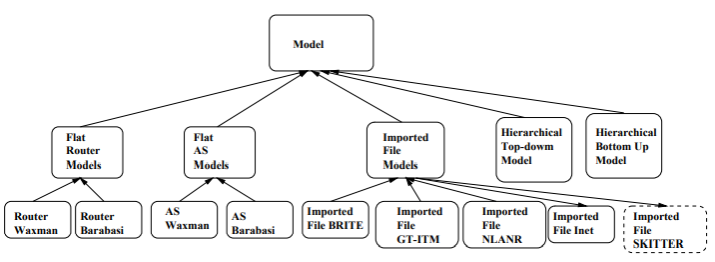
\includegraphics[width=1\textwidth]{img/teoria/brite.PNG}
    \caption{Modelos soportados por \acrshort{brite} \cite{brite}}
    \label{fig:brite}
\end{figure}

\vspace{3mm}

En el caso del Router Waxman, como su nombre indica, emplea un modelo de probabilidad Waxman para establecer la Interconexión de los nodos en la topología \cite{brite_zegura}:

\[P_{\text{Waxman}}(u,v) = \alpha \cdot e^{-\frac{d}{\beta \cdot L}}\]
    
    Donde:
\begin{itemize}
    \renewcommand{\labelitemi}{}
    \item \textit{P(u,v)} es la probabilidad en función de la distancia euclidiana entre un nodo \textit{u} y un nodo \textit{v} de la red.
    \item $\alpha$ es un parámetro específico del modelo que hace referencia a la densidad de enlaces y toma generalmente un valor igual a 0.2.
    \item $\beta$ es un parámetro específico del modelo que hace referencia al ratio enlaces largos/enlaces cortos en la topología y toma generalmente un valor igual a 0.15.
    \item \textit{L} es la máxima distancia entre dos nodos cualesquiera.
\end{itemize}

\vspace{3mm}

Por otro lado, el modelo Router Barabasi-Albert está basado en la generación de topologías con un incremento exponencial del número de nodos a lo largo del tiempo. Además, se permite una conexión preferencial, suponiendo que cuanto mayor grado de conectividad abarque un nodo, mayor será la probabilidad de que este añada nuevos enlaces. Por lo tanto, el plano de la topología comienza con un número de nodos inicial \textit{N0} y se van añadiendo los demás uno a uno. Cada uno de estos nuevos nodos se conectará a \textit{N} nodos ya añadidos a la topología con una probabilidad \cite{brite_zegura}:

\[P_{\text{Barabási-Albert}}(k_i) = \frac{k_i}{\sum_{j}^{}k_j}\]
    
    Donde:
\begin{itemize}
    \renewcommand{\labelitemi}{}
    \item \textit{P(k)} es la probabilidad de conexión del nodo \textit{i} con grado \textit{k}.
    \item $\sum_{j}^{}k_j$ es el sumatorio de los grados de todos los nodos de la topología.
\end{itemize}

\subsubsection{Automatización de la ejecución}
\label{sec:brite_eje}

A modo de facilitar la ejecución de la herramienta \gls{brite} se aporta en el repositorio el fichero de python \textit{generador\_brite.py}, dedicado a la automatización del proceso de creación de un fichero de configuración. Este recibirá los parámetros de entrada que caracterizarán a la topología a generar (ver Sección \ref{sec:param}) y escribirá el nuevo fichero.

\vspace{3mm}

También, se añade el fichero de python \textit{parser.py}, que se encargará de definir la función de transformación del archivo de salida proporcionado por \gls{brite} (en formato .brite) en dos nuevos ficheros: \textit{Nodos.txt} y \textit{Enlaces.txt}. Respectivamente, estos almacenarán las posiciones x e y de los nodos en el plano y la información sobre las distancias y los identificadores de los nodos que se interconectan con cada enlace. Este funcionamiento se muestra de forma gráfica en la Figura \ref{fig:parser}.

\vspace{3mm}

\begin{figure}[H]
    \centering
    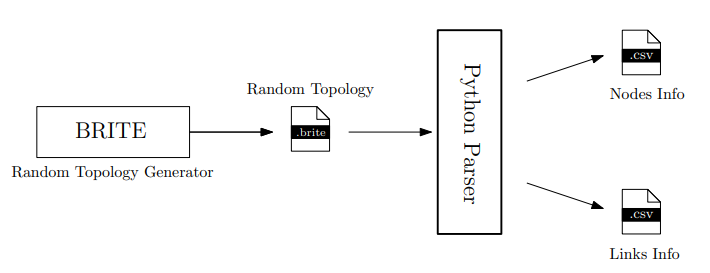
\includegraphics[width=0.7\textwidth]{img/teoria/parser.png}
    \caption{Esquema de funcionamiento de \acrshort{brite} y del \textit{parser} \cite{den2ne}}
    \label{fig:parser}
\end{figure}

\vspace{3mm}

Teniendo en cuenta los ficheros anteriores, se proporciona un script \textit{autogenerador.sh} donde se incluyen todas sus funcionalidades y se automatiza todo el proceso de ejecución de la herramienta. Este script sigue la siguiente secuencia de pasos:

\begin{enumerate}
    \item Define los valores de cada uno de los parámetros de entrada.
    \item Ejecuta el fichero de python \textit{generador\_brite.py} aplicando los parámetros definidos para el modelo Waxman y Barabasi.
    \item Genera 10 topologías diferentes para cada archivo de configuración a partir de 10 ficheros de semillas (\textit{seed\_files}) dados en el repositorio. Esto posibilita la generación de 10 topologías totalmente diferentes para cada escenario de red definido (a partir de unos mismos parámetros de entrada). 
    \item Se aplica un bucle en función del número de semilla:
    \begin{enumerate} 
        \item Crea el directorio para cada escenario y se ejecuta la heramienta \gls{brite} sobre cada uno.
        \item Se ejecuta \textit{parser.py} para obtener a la salida los ficheros \textit{Nodos.txt} y \textit{Enlaces.txt} de cada uno de los escenarios.   
    \end{enumerate} 
\end{enumerate}



